\section{IPv6 adresace}
\label{sec:ipv6-adresace}
Stejně jako IPv4 slouží IPv6 adresace k logické adresaci síťových prvků v internetu, ale i na lokální síti.
IPv6 adresace byla vytvořeno jako náhrada IPv4 z důvodu nedostatku adres.
Tato adresace není s IPv4 zaměnitelná a proto je nutné tyto adresy překládat nebo je zabudovat do této adresy.
Komunikace se po obdržení IPv6 adresy řídí pomocí směrování.
IPv6 adresa se skládá z 128 bitů pomocí 16 oktetů.
\[\mathlarger{\mathlarger{\mathlarger{\mathlarger{2001:0db8:3c4d:0000:0000:a011:0000:0000}}}}\]
Zápis adresy je možné zkrátit odstraněním nulových oktetů.
\[\mathlarger{\mathlarger{\mathlarger{\mathlarger{2001:db8:3c4d::a011:0:0}}}}\]
Je možné takto adresu zkrátit pouze jednou.
Takových adres může existovat několik trilionů.
Po uživatelovi není pro funkci potřeba žádná konfigurace.
Tento protokol musí podporovat akorát poskytovatel internetového připojení.
\subsection{Porovnání s IPv4}
\begin{itemize}
  \item Větší adresní prostor
  \item Zjednodušuje změnu adresy při změně poskytovatele pomocí změny pouze části prefixu.
  \item Zjednodušuje správu velkých sítí
  \item Součástí IPv6 je i šifrování
\end{itemize}
\subsection{Adresace}
Samotná adresa se skládá z části pro prefix a částí pro indentifikaci síťového rozhraní.
Obě tyto části zaujímají přesně polovinu adresy.
Jelikož indentifikace síťového rozhraní je celosvětově unikátní, tak se tato adresa s časem mění.
Na lokální síti se využívá specifikace EUI64 pro generování adres pomocí MAC.
\subsection{Speciální adresy IPv6}
\begin{description}
  \item[Unicast]- Unicast adresa je adresa, která se používá pro komunikaci s jedním zařízením.
  \item[Multicast]- Multicast adresa je adresa, která se používá pro komunikaci se skupinou.
  \item[Anycast]- Anycast adresa je adresa, která se používá pro komunikaci s kýmkoli v zadané skupině.
\end{description}
Broadcast v IPv6 neexistuje. ::0 je pro zařízení bez rozhraní a ::1 slouží jako loopback.
\subsection{IPv6 Paket}
Sturktura paketu se oproti IPv4 změnila tím, že záhlaví je povinné můžeme za něj přidat volitelná záhlaví určené pro svůj stanovaný účel.\\
\begin{center}
  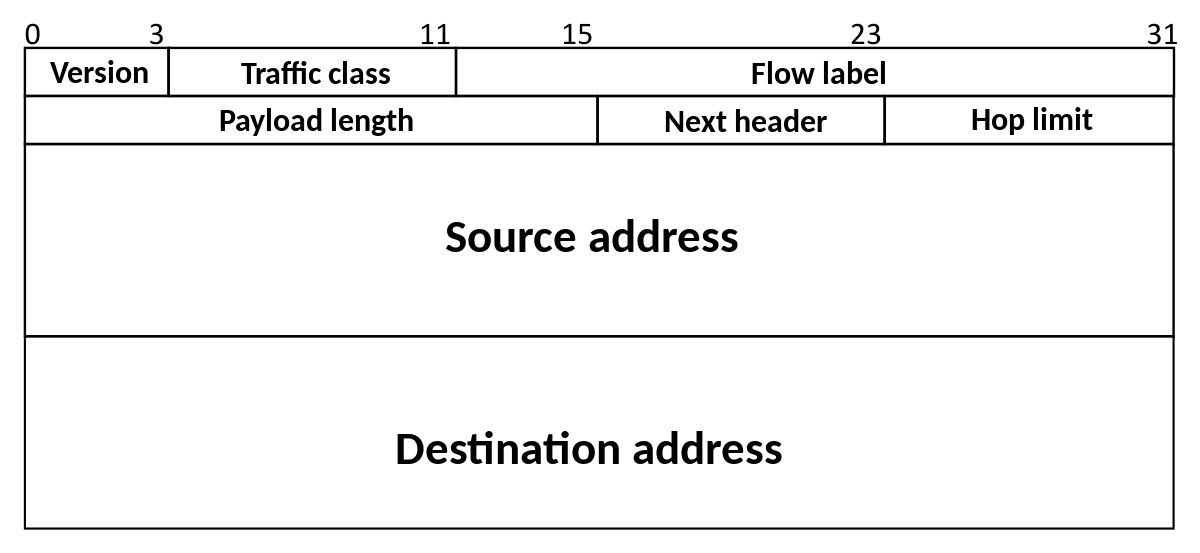
\includegraphics[width=0.7\linewidth]{TVY-POS/IPv6-adresace/IPv6_paket.png}\\
  Traffic class = priorita | Flow label = způsob zacházení s paketem | Payload lenght = Délka dat
\end{center}
